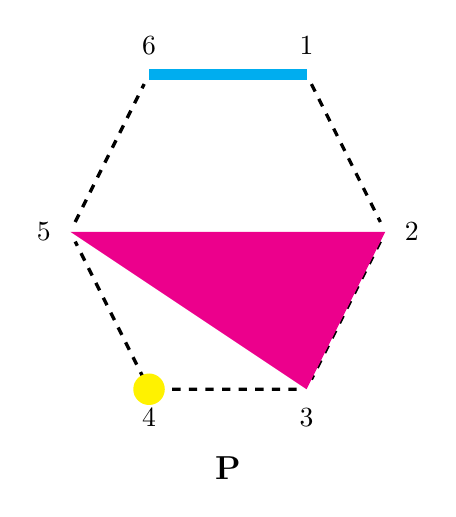
\begin{tikzpicture}[scale=1]
    \node at (3,0) {\large $\mathbf{P}$};
    \node [label = above : {$1$}] (1)
        at (4,5) {};
    \node [label = right : {$2$}] (2)
        at (5,3) {};
    \node [label = below : {$3$}] (3)
        at (4,1) {};
    \node [label = below : {$4$}] (4)
        at (2,1) {};
    \node [label = left : {$5$}]  (5)
        at (1,3) {};
    \node [label = above : {$6$}] (6)
        at (2,5) {};
    \draw [dashed][very thick]
    (1) -- (2) -- (3) -- (4)
        -- (5) -- (6) -- (1);
    \fill [color = magenta] (5,3) -- (4,1)
        -- (1,3) -- cycle;
    \draw [color = cyan][line width = 4pt] 
        (4,5) -- (2,5);
    \fill [color=yellow] (2,1) circle (0.2);
  \end{tikzpicture}